\documentclass{article}
\usepackage{tikz, comment}
\usepackage{pifont}
\usepackage{fontspec}
\usetikzlibrary{arrows, decorations.markings, decorations.pathreplacing}
\begin{comment}
:Title: Not defined yet
:Tags: vertices;slope;rule;polygon;limit;length;functions
:Author: Prof.Hu Ji-shan, HKUST
:Slug: No name yet

Description Here.........
\end{comment}
\begin{document}\centering

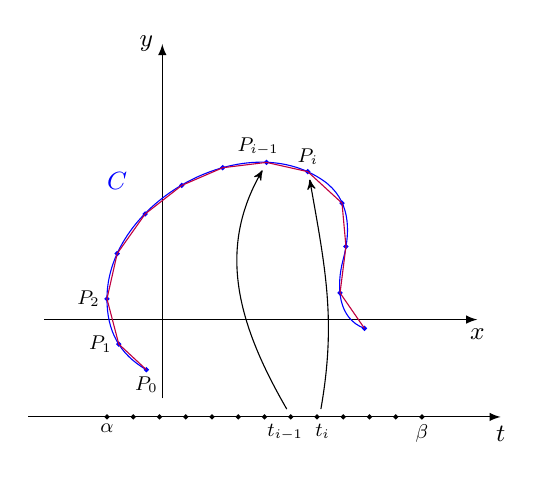
\begin{tikzpicture}[>=latex, xscale=.5*1, yscale=.5*1] [font=\sf\small]

\draw[->] (-3, 0) -- (8, 0)node[below] {\small $x$} ;
\draw[->] (0, -2) -- (0, 7)node[left] {\small $y$};

\begin{scope}[rotate=0, xshift = -40, yshift = 15]
\draw[blue] (1, -1.8) to [out=150, in=-90 ] (0,0) to [out=90,in=145] (5.5,3) to [out=-35,in=75] (6,1) to [out=-105,in=160] (6.54, -0.75);

\draw[blue, fill] (1, -1.8) circle(0.05) node[black, below, scale=0.8] {$P_0$};
\draw[blue, fill] (0.3, -1.15) circle(0.05) node[black, left, scale=0.8] {$P_1$};
\draw[blue, fill] (0, 0) circle(0.05) node[black, left, scale=0.8] {$P_2$};
\draw[blue, fill] (0.26, 1.15) circle(0.05);
\draw[blue, fill] (0.97, 2.155) circle(0.05);
\draw[blue, fill] (1.9, 2.88) circle(0.05);
\draw[blue, fill] (2.94, 3.33) circle(0.05);
\draw[blue, fill] (4.05, 3.465) circle(0.05) node[black, above, xshift=-3, scale=0.8] {$P_{i-1}$};

\draw[blue, fill] (5.1, 3.23) circle(0.05) node[black, above, scale=0.8] {$P_{i}$};
\draw[blue, fill] (5.97, 2.43) circle(0.05);
\draw[blue, fill] (6.07, 1.33) circle(0.05);
\draw[blue, fill] (5.92, 0.15) circle(0.05);
\draw[blue, fill] (6.54, -0.75) circle(0.05);

\draw[purple] (1, -1.8)--(0.3, -1.15)--(0, 0)--(0.26, 1.15)--(0.97, 2.155)--(1.9, 2.88)--(2.94, 3.33)--(4.05, 3.465)--(5.1, 3.23)--(5.97, 2.43)--(6.07, 1.33)--(5.92, 0.15)--(6.54, -0.75);

\node[blue] at (0.26, 3) {$C$};

\foreach \t in {0,1,2,...,12}
\draw[fill] ({0+(\t)*8/12}, {-3}) circle(0.05);
\draw[->] (-2, -3) -- (10, -3)node[below] {\small $t$} ;
\node[below, scale=0.8] at ({0}, {-3}) {$\alpha$};
\node[below, scale=0.8] at ({0+(12)*8/12}, {-3}) {$\beta$};
\node[below, xshift=-2, scale=0.8] at ({0+(7)*8/12}, {-3}) {$t_{i-1}$};
\node[below, xshift= 2, scale=0.8] at ({0+(8)*8/12}, {-3}) {$t_i$};

\draw[->, >=stealth'] ({0+(7)*8/12-0.1}, {-3+0.2}) to [out=120,in=240] ({4.05-0.1}, {3.465-0.2});
\draw[->, >=stealth'] ({0+(8)*8/12+0.1}, {-3+0.2}) to [out=80,in=-80] ({5.1+0.05}, {3.23-0.2});

\end{scope}

\end{tikzpicture}
\end{document}